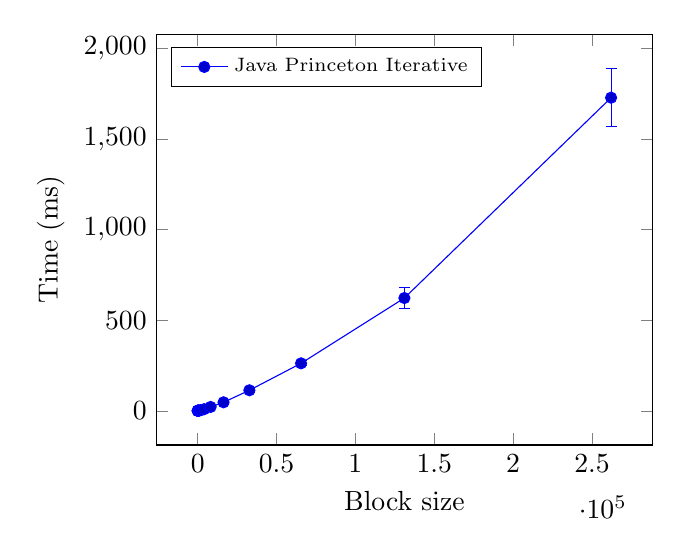
\begin{tikzpicture}
\begin{axis}[xlabel={Block size},ylabel={Time (ms)},width=0.65\linewidth,legend pos=north west,scaled y ticks = false,legend cell align=left,legend style={font=\scriptsize}]
\addplot+[error bars/.cd, y dir=both,y explicit] coordinates {
(16, 0.1398) +- (0.1496, 0.1496)
(32, 0.0492) +- (0.0139, 0.0139)
(64, 0.1078) +- (0.0326, 0.0326)
(128, 0.1991) +- (0.0359, 0.0359)
(256, 0.3547) +- (0.1008, 0.1008)
(512, 0.7740) +- (0.1657, 0.1657)
(1024, 1.7228) +- (0.2675, 0.2675)
(2048, 3.8546) +- (0.7268, 0.7268)
(4096, 8.8053) +- (1.9485, 1.9485)
(8192, 21.1757) +- (4.9079, 4.9079)
(16384, 46.8150) +- (9.6619, 9.6619)
(32768, 113.1953) +- (11.0218, 11.0218)
(65536, 261.9954) +- (13.8293, 13.8293)
(131072, 622.4328) +- (57.9001, 57.9001)
(262144, 1728.4640) +- (161.0712, 161.0712)
};
\legend{Java Princeton Iterative}
\end{axis}
\end{tikzpicture}
